\documentclass[conference]{IEEEtran}
\usepackage{amsmath,amssymb,graphicx,booktabs,url}
\usepackage{newtxtext,newtxmath}
\usepackage[hidelinks]{hyperref}
\graphicspath{{figures/}}
% Generated from audited CSV by scripts/analyze_ngan.py. Do not edit numbers.
\newcommand{\TrialCount}{1308}
\newcommand{\OkCount}{1308}
\newcommand{\InputCount}{69}
\newcommand{\GroupCount}{436}
\newcommand{\CompleteCount}{436}
\newcommand{\FailureCount}{0}
\newcommand{\QuickTimeMillion}{4,454.79}
\newcommand{\QuickMemMillion}{0.001831}
\newcommand{\QuickGrowth}{178.3}
\newcommand{\MergeTimeMillion}{3,783.97}
\newcommand{\MergeMemMillion}{7.630184}
\newcommand{\MergeGrowth}{210.7}
\newcommand{\HeapTimeMillion}{4,790.74}
\newcommand{\HeapMemMillion}{0.000210}
\newcommand{\HeapGrowth}{306.3}
\newcommand{\RadixTimeMillion}{1,760.36}
\newcommand{\RadixMemMillion}{15.268597}
\newcommand{\RadixGrowth}{224.2}
\newcommand{\MergeBytesPerElement}{8.001}
\newcommand{\RunGainRandom}{3.0}
\newcommand{\RunGainSorted}{91.6}
\newcommand{\RunGainReverse}{57.0}
\newcommand{\RunGainSmallMin}{-21.6}
\newcommand{\RunGainSmallMax}{89.6}
\newcommand{\RunGainLargeMin}{-9.8}
\newcommand{\RunGainLargeMax}{91.6}
\newcommand{\MemoryTableRows}{10,000 & 1.22 [1.19, 1.25] & 78.75 [78.75, 78.75] & 0.21 [0.21, 0.21] & 166.20 [166.20, 166.20] \\
50,000 & 1.41 [1.38, 1.47] & 391.31 [391.31, 391.31] & 0.21 [0.21, 0.21] & 791.29 [791.29, 791.29] \\
100,000 & 1.62 [1.53, 1.62] & 781.96 [781.96, 781.96] & 0.21 [0.21, 0.21] & 1,572.54 [1,572.54, 1,572.54] \\
500,000 & 1.78 [1.69, 1.84] & 3,907.03 [3,907.03, 3,907.03] & 0.21 [0.21, 0.21] & 7,822.54 [7,822.54, 7,822.54] \\
1,000,000 & 1.88 [1.81, 2.06] & 7,813.31 [7,813.31, 7,813.31] & 0.21 [0.21, 0.21] & 15,635.04 [15,635.04, 15,635.04] \\}
\newcommand{\CoverageTableRows}{RQ1 & 180 & 180 & 0 \\
RQ2 & 720 & 720 & 0 \\
RQ3 & 840 & 840 & 0 \\}
\newcommand{\CountTableRows}{Quick & 184,161 & 269,435 & 68,974 & 26,542,114 & 38,211,290 & 10,029,524 \\
Merge & 120,420 & 387,652 & 277,232 & 18,673,907 & 58,576,755 & 40,902,848 \\
Heap & 235,326 & 260,324 & 139,123 & 36,793,761 & 39,293,759 & 20,548,417 \\
Radix & -- & 202,040 & 172,044 & -- & 20,002,040 & 17,002,044 \\}
\newcommand{\DistributionTableRows}{D1 & Radix & 1,760.36 & 2.72 \\
D2 & Radix & 2,117.03 & 1.57 \\
D3 & Radix & 2,034.24 & 1.63 \\
D4 & Radix & 2,092.69 & 1.64 \\
D5 K=1000 & Radix & 728.08 & 5.25 \\
D5 K=10 & Radix & 675.89 & 5.73 \\
D5 K=2 & Radix & 695.26 & 5.72 \\
D6 R=2 & Radix & 2,096.34 & 4.18 \\
D6 R=16 & Radix & 2,358.75 & 2.05 \\
D6 R=256 & Radix & 1,952.50 & 2.34 \\}
\newcommand{\AdaptiveTableRows}{D1 & 4,454.79 & 3,783.97 & 3,094.37 & 3,190.32 & 330.39 \\
D2 & 2,874.41 & 3,331.86 & 151.16 & 1,801.60 & 60.79 \\
D3 & 2,659.78 & 3,325.42 & 1,634.39 & 2,642.36 & 70.25 \\
D4 & 2,783.76 & 3,430.82 & 1,867.51 & 4,345.03 & 67.10 \\
D5 K=1000 & 3,822.33 & 2,525.27 & 2,595.84 & 2,563.58 & 139.41 \\
D5 K=10 & 3,872.30 & 2,405.35 & 2,592.83 & 2,361.51 & 82.28 \\
D5 K=2 & 3,973.54 & 2,359.70 & 1,764.06 & 1,765.41 & 49.08 \\
D6 R=2 & 8,760.56 & 3,115.26 & 423.11 & 1,586.64 & 105.13 \\
D6 R=16 & 4,262.94 & 2,932.16 & 923.42 & 1,976.44 & 190.78 \\
D6 R=256 & 3,918.54 & 3,067.78 & 1,487.09 & 2,158.75 & 235.94 \\}
\newcommand{\MechanismTableRows}{D1 & Adaptive & 18,599,873 & 16,130 & 3.814968 \\
D1 & noA & 18,588,462 & -- & 3.814968 \\
D2 & Adaptive & 999,999 & 1 & 0.000141 \\
D2 & noA & 11,032,952 & -- & 3.814968 \\
D4 & Adaptive & 5,239,742 & 233 & 3.804775 \\
D4 & noA & 12,015,805 & -- & 3.814968 \\
D6 R=2 & Adaptive & 1,999,998 & 2 & 3.815166 \\
D6 R=2 & noA & 11,541,147 & -- & 3.814968 \\}

\title{An Empirical Study of Classical Sorting Algorithms and Powersort on Partially Ordered Integer Data}
\author{\IEEEauthorblockN{My, Ngan, Hai, Thien, and Dan}
\IEEEauthorblockA{Group 1 --- CSD203 FA26}}
\begin{document}
\maketitle
\begin{abstract}
Sorting performance depends on input structure, implementation details, and the resource being measured. This study compares pure-Python implementations of Quicksort, top-down Mergesort, Heapsort, four-pass least-significant-digit Radix sort, and an adaptive mergesort using the Powersort merge policy. A variant without natural-run detection isolates the contribution of run adaptation, while Python's built-in sorted function provides a library reference. Experiments cover six controlled data families, ten distribution configurations, input sizes from ten thousand to one million integers, and three deterministic seeds. Time, additional allocation, and operation counts are obtained in separate processes; every completed output is compared in full with an independent sorted result. The recorded matrix contains \TrialCount{} trials, of which \OkCount{} pass output validation. The memory analysis distinguishes asymptotic auxiliary space from the additional allocations observed by tracemalloc. Generated tables and figures are derived from the retained raw CSV after source, configuration, checksum, seed, and unit checks. Conclusions apply to the measured implementations and workstation, rather than to all implementations of these algorithms or to an end-to-end AI pipeline.
\end{abstract}
\begin{IEEEkeywords}
sorting algorithms, auxiliary memory, Powersort, reproducible experiments, partially ordered data
\end{IEEEkeywords}

\section{Introduction}
Data-processing pipelines often combine identifiers, time-ordered logs, and batches sorted independently. The resulting order can differ substantially from a uniformly random array. A comparison must consider both input size and structure while supplying equivalent data to competing algorithms.

RQ1 asks how time and additional memory change with input size for Quick, Merge, Heap, and Radix on random integers. RQ2 asks whether input distribution changes their relative performance. RQ3 compares adaptive Powersort with Quick, Merge, a no-run-detection variant (noA), and the library reference. The five-person scope omits galloping and a second ablation; it retains natural runs, minrun extension, binary insertion, and the Powersort merge policy.

We distinguish a prediction, a validated output, and a measured performance result. An $N\log N$ model does not predict an exact wall-clock multiplier. A successful unit test does not establish a timing ranking. A fixed number of Radix passes does not imply identical elapsed time under every distribution.

\section{Algorithms and Implementations}
Measurements use repository revision \texttt{c73bc10}. Algorithm and benchmark source files were unchanged during the experiment. The full revision and SHA-256 file hashes accompany the raw results.

\subsection{Quick, Heap, and Radix}
Quick uses Hoare partitioning, a median-of-three pivot, recursion, and no insertion cutoff~\cite{hoare}. It shares helpers with its counted path. Passing \texttt{None} disables updates, but helper calls and counter-condition branches remain in the timed path. Timing includes this implementation overhead. The recursion limit is not raised.

Heap follows the classical heapsort family~\cite{williams}, builds a max-heap bottom-up, and performs iterative sift-down using a hole and a retained element. It uses a constant number of auxiliary variables rather than an auxiliary array: $O(1)$ auxiliary space in the usual word model, not a guaranteed zero-byte allocation.

Radix uses base 256 and four stable counting passes on $[0,2^{31}-1]$. Each pass counts digits, accumulates bucket positions, places elements from right to left into an $N$-element output buffer, and copies back. Extra space is $\Theta(N+256)$. Updating the input list is an interface property, not a claim of constant space. The normal path uses slice assignment for copy-back; the counted path represents this by explicit element reads and writes. Counts describe logical array traffic, not every internal CPython memory access.

\subsection{Stable Top-down Merge Sort}
Ngan's implementation divides half-open intervals $[lo,hi)$ at $\lfloor(lo+hi)/2\rfloor$, recursively sorts the children, and merges back. \texttt{sort} allocates a single list of $N$ references for $N\geq2$; \texttt{\_sort} and \texttt{\_merge} reuse it throughout recursion. No input slicing, per-child array allocation, cutoff, or already-sorted shortcut is used. This follows the reusable-buffer top-down merge pattern~\cite{merge}.

The right value is selected only if strictly smaller than the left. Otherwise the left value is selected. Assuming sorted children, choosing the smallest remaining head preserves the sorted output prefix. Copying the remainder preserves every element. Induction on interval length establishes a sorted permutation. Taking equal keys from the left first preserves their original relative order, establishing stability under a consistent key ordering.

The recurrence is
\[
T(N)=T(\lfloor N/2\rfloor)+T(\lceil N/2\rceil)+\Theta(N).
\]
All merge levels execute even on sorted input. Time is $\Theta(N\log N)$ for these fixed-width keys. The buffer needs $\Theta(N)$ reference slots, and recursion has $O(\log N)$ depth. It stores references to existing integers rather than cloning their objects.

The counted path uses the same splits and comparisons. Reads and writes to both lists include the initial $N$ buffer-slot writes; scalar arithmetic and recursion bookkeeping are excluded. Tests cover 1,000 deterministic fuzz inputs, stability on 1,000 key-only records, comparison traces, buffer identity, and absence of input slicing. Key-only comparison separates the ordering key from the record payload, as illustrated by the textbook's companion sorting examples~\cite{goodrich}.

The essential merge procedure is: copy $a[lo:hi)$ into the shared
buffer; set $i=lo$ and $j=mid$; for each destination $k$ from $lo$ to
$hi-1$, take the remaining left head if the right child is exhausted,
otherwise take the right head if the left child is exhausted or its key
is strictly smaller; in every other case take the left head. Advance
only the selected cursor. Here the interval notation describes indices;
the implementation copies with a loop, not a Python slice.

\subsection{Adaptive Powersort and noA}
The adaptive implementation scans increasing or strictly decreasing runs. Strictly decreasing runs are reversed without reversing equal-key order. Short runs are extended to minrun by stable binary insertion. \texttt{node\_power}, \texttt{\_push\_run}, and \texttt{\_merge\_at} implement Powersort scheduling; each merge buffers the shorter child~\cite{powersort,listsort}.

NoA disables natural-run recognition, sorts consecutive minrun-sized blocks, then uses the same merging machinery. The ablation measures the net effect of run detection and avoided work, not the isolated cost of one scan. The simplified implementation does not reproduce all CPython optimizations. The library reference calls \texttt{sorted(a)} in C and includes its returned-list allocation.

\section{Experimental Method}
\subsection{Inputs and Matrix}
D1 contains pseudorandom integers from a local seeded generator. D2 sorts D1; D4 reverses D2. D3 performs $\lfloor N/1000\rfloor$ swaps of distinct positions in D2 with a separate stream seeded by seed$+10000$. D5 selects from a pool of $K$ distinct values, $K\in\{1000,10,2\}$. D6 splits D1 into $R\in\{2,16,256\}$ balanced consecutive batches, sorts each, and concatenates them. A generated batch count is not necessarily the natural-run count.

RQ1 uses D1 at $N=10{,}000$, $50{,}000$, $100{,}000$, $500{,}000$, and $1{,}000{,}000$. RQ2/RQ3 use all ten configurations at $N=100{,}000$ and $1{,}000{,}000$. Seeds are 2026, 2027, and 2028. Each configuration has separate time, memory, and count trials; the library has only time/memory. Shared trials are measured once and assigned to each applicable RQ.

\subsection{Environment and Measurement Boundary}
CPython 3.12.14 runs on the available Windows 11 workstation with 12 logical CPUs and 15.3 GiB physical memory as reported by the recorder. This is Ngan's development workstation, not a claim that the designated Hai machine was used. CPU identifier, OS build, executable path, and source hashes are retained. Power state, temperature, and unrelated background applications were not fully controlled.

Workers run sequentially. Input generation, SHA-256, a warm-up on at most 1,000 elements of the same family, and the working copy precede measurement. Garbage collection keeps its default setting. \texttt{perf\_counter\_ns} brackets the sort call. A separate worker records peak additional allocation with \texttt{tracemalloc}; tracing ends before oracle construction. Preparation, validation, and CSV writing are excluded.

The 60-second limit covers the entire worker, including preparation and validation. A timeout retains its phase and is not reported as a completed 60-second sort. Out-of-memory status requires an observed memory exception. Incorrect and incomplete trials remain in the raw CSV but are excluded from performance estimates.

\subsection{Validation and Aggregation}
Completed outputs are compared in full with \texttt{sorted(input)}. Input SHA-256 uses unsigned 32-bit little-endian values. The output checksum is $h_0=0$,
\[
h_{i+1}=(31h_i+x_i)\bmod 2^{64}.
\]
A separate audit regenerates \InputCount{} inputs, recomputes hashes and sorted-output checksums independently of the worker checksum helpers, checks configuration coverage, rejects duplicates, and verifies source/environment identity.

We report median, minimum, maximum, and successful count over three seeds. These are different deterministic inputs, not repeated timings of one input; min--max ranges are not confidence intervals. Complete groups have all three successful seeds. Throughput is $N/\mathrm{elapsed\_ms}$ thousand elements/s. KiB is 1024 bytes and MiB is $2^{20}$ bytes. Ratios compare medians under identical conditions.

\section{Results}
\subsection{Coverage}
Table~\ref{tab:coverage} counts trials by RQ; shared trials occur in multiple rows. There are \TrialCount{} distinct trials, \OkCount{} validated outputs, and \FailureCount{} other outcomes. Of \GroupCount{} configuration--mode groups, \CompleteCount{} contain three successful seeds. The source is \texttt{results/raw/ngan\_20261029.csv}; no earlier illustrative or sample CSV is used.

\begin{table}[t]
\caption{Trial coverage by research question}\label{tab:coverage}
\centering\begin{tabular}{lrrr}\toprule
Question & Attempted & Validated & Other status\\\midrule
\CoverageTableRows
\bottomrule\end{tabular}
\end{table}

\subsection{RQ1: Memory and Input Size}
Table~\ref{tab:memory} compares the four baseline implementations. At one million integers, Merge's median is \MergeMemMillion{} MiB, or \MergeBytesPerElement{} measured bytes per element. This is consistent with a linear reference buffer and smaller interpreter overhead. It is not the total integer-input size, process resident memory, or a universal cost across Python builds.

Quick's median is \QuickMemMillion{} MiB, Heap's is \HeapMemMillion{} MiB, and Radix's is \RadixMemMillion{} MiB. Quick has recursive temporary state despite lacking an auxiliary array. Heap keeps small iterative state. Radix's output buffer, bucket arrays, and copy-back distinguish it from a constant-space algorithm.

\begin{table*}[t]
\caption{RQ1 additional allocation on D1 in KiB: median [minimum, maximum]. Partial groups explicitly show the successful count.}\label{tab:memory}
\centering\small
\begin{tabular}{rllll}\toprule
$N$ & Quick & Merge & Heap & Radix\\\midrule
\MemoryTableRows
\bottomrule\end{tabular}
\end{table*}

\begin{figure}[t]\centering
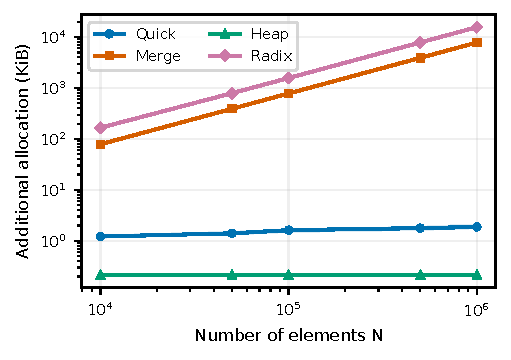
\includegraphics[width=\columnwidth]{rq1_memory.pdf}
\caption{RQ1 memory: medians and three-seed min--max bands. Both axes are logarithmic. Only complete groups are plotted.}\label{fig:memory}
\end{figure}

At one million elements, median times are \QuickTimeMillion{} ms (Quick), \MergeTimeMillion{} ms (Merge), \HeapTimeMillion{} ms (Heap), and \RadixTimeMillion{} ms (Radix). From $10^4$ to $10^6$, their time multipliers are \QuickGrowth{}, \MergeGrowth{}, \HeapGrowth{}, and \RadixGrowth{}. These implementation-level observations do not prove asymptotic bounds or universal rankings. The initial hypothesis that Quick would precede Merge, Heap, and Radix at small sizes is contradicted by the $N=10{,}000$ measurements, where Radix is fastest among these four. We retain this outcome rather than treating the initial ranking as a requirement. Linear logical work also does not force a 100-fold wall-clock increase across a 100-fold input-size increase.

\begin{figure}[t]\centering
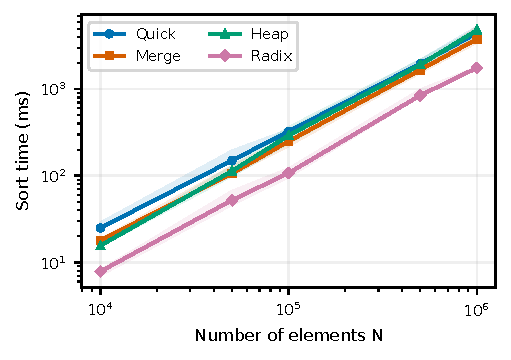
\includegraphics[width=\columnwidth]{rq1_time.pdf}
\caption{RQ1 timing on D1. Separate workers measure timing, memory, and operations. Bands are min--max ranges, not confidence intervals.}\label{fig:time}
\end{figure}

Table~\ref{tab:counts} provides a second view of scaling through logical
operation counts. Radix avoids key-to-key comparisons, so its comparison
entry is undefined rather than a measured zero. Quick, Merge and Heap
have different comparison and array-access totals even though their
typical time models are of the same order. These totals should not be
converted to elapsed time with a shared per-operation constant.
\begin{table*}[t]
\caption{RQ1 median logical counts on D1; three seeds per cell. C: key comparisons, R: array reads, W: array writes.}
\label{tab:counts}\centering\small
\begin{tabular}{lrrrrrr}\toprule
 & \multicolumn{3}{c}{$N=10{,}000$} & \multicolumn{3}{c}{$N=1{,}000{,}000$}\\
Algorithm & C & R & W & C & R & W\\\midrule
\CountTableRows
\bottomrule\end{tabular}
\end{table*}

\subsection{RQ2: Input Distribution}
Figure~\ref{fig:distribution} divides each median by the fastest of the four baseline medians for the same condition. One identifies the fastest measured implementation. This normalization does not imply equal absolute time across distributions. Table~\ref{tab:winners} gives absolute winning times at one million elements and slowest-to-fastest ratios.

\begin{figure*}[t]\centering
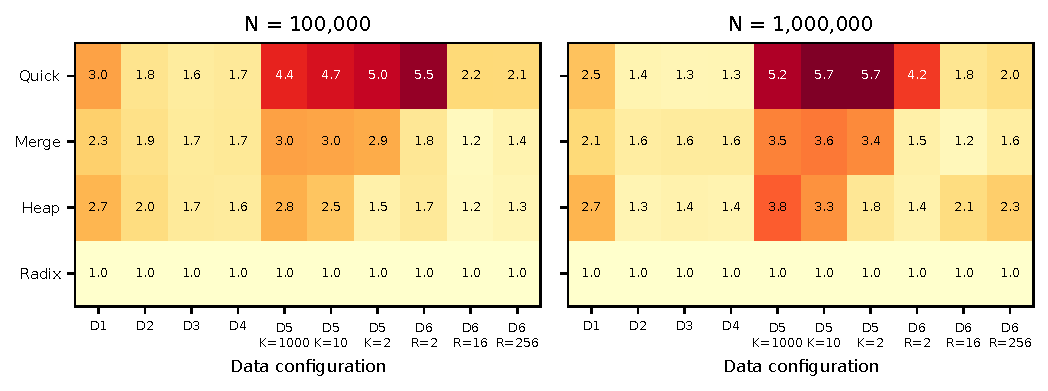
\includegraphics[width=.98\textwidth]{rq2_relative_time.pdf}
\caption{RQ2 median time relative to the fastest baseline in each column. Larger numbers mean slower execution.}\label{fig:distribution}
\end{figure*}

\begin{table}[t]
\caption{RQ2 at $N=1{,}000{,}000$: fastest baseline and timing spread}\label{tab:winners}
\centering\small\begin{tabular}{llrr}\toprule
Input & Fastest & Time (ms) & Slow/fast\\\midrule
\DistributionTableRows
\bottomrule\end{tabular}
\end{table}

For fixed $N\geq2$, the reviewed Radix counter gives $20N+2040$ logical reads and $17N+2044$ writes, including buffer initialization. An instrumented in-memory copy of the normal path and the count records check these formulas. Invariant counts do not guarantee invariant elapsed time or traced allocation. Python operations, allocation behavior, cache effects, and scheduling may contribute; this experiment does not isolate their causes.

Radix has the lowest median of the four baselines in every measured
configuration at one million elements. Its D5 timings are lower than
its D1 timing despite identical logical traffic at fixed size. Quick's
largest median in this table occurs for D6 with two batches, exceeding
its random-input median. Thus ``partially sorted'' alone is insufficient
to predict an improvement for every implementation. Stability and the
additional buffer cost still matter when selecting Radix over Heap.

\subsection{RQ3: Natural-run Adaptation}
Table~\ref{tab:adaptive} compares the adaptive implementation with Quick,
Merge, noA, and the library on all ten configurations at one million elements.
The smaller-size results are retained in the accompanying summary CSV.
\begin{table*}[t]
\caption{RQ3 median sort time at $N=1{,}000{,}000$ in ms. Complete cells use three seeds.}
\label{tab:adaptive}
\centering\small\begin{tabular}{lrrrrr}\toprule
Input & Quick & Merge & Adaptive & noA & Library\\\midrule
\AdaptiveTableRows
\bottomrule\end{tabular}
\end{table*}
The ablation computes
\[
100\,\frac{T_{\mathrm{noA}}-T_{\mathrm{adaptive}}}{T_{\mathrm{noA}}}.
\]
Positive values mean adaptive sorting is faster; negative values are retained. At one million elements, reductions are \RunGainRandom{}\% on D1, \RunGainSorted{}\% on D2, and \RunGainReverse{}\% on D4. Across distributions, reductions range from \RunGainSmallMin{}\% to \RunGainSmallMax{}\% at $N=100{,}000$, and \RunGainLargeMin{}\% to \RunGainLargeMax{}\% at $N=1{,}000{,}000$.

\begin{figure}[t]\centering
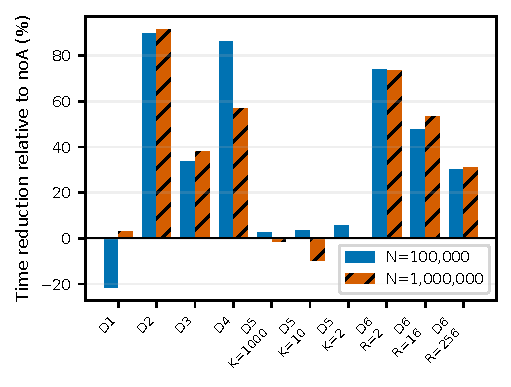
\includegraphics[width=\columnwidth]{rq3_ablation.pdf}
\caption{RQ3 median time reduction relative to noA. The zero line separates improvements from regressions.}\label{fig:ablation}
\end{figure}

NoA provides the internal control for run adaptation. A gap to the built-in library combines Python-versus-C execution, library optimizations including galloping, and output-allocation differences; it cannot be assigned solely to Powersort. Run statistics describe runs scanned before minrun extension. Absorbed portions are not rescanned, so mean run length need not equal $N/\mathrm{run\_count}$.

Table~\ref{tab:mechanism} provides operation and memory evidence for four
contrasting conditions: random, sorted, reverse-sorted, and two sorted batches.
Run counts are not defined for noA. All other configurations are retained in
the summary CSV rather than omitted from the experiment.
\begin{table}[t]
\caption{RQ3 mechanism evidence at $N=1{,}000{,}000$: medians over three seeds}
\label{tab:mechanism}
\centering\footnotesize\setlength{\tabcolsep}{3pt}
\begin{tabular}{llrrr}\toprule
Input & Variant & Comparisons & Runs & MiB\\\midrule
\MechanismTableRows
\bottomrule\end{tabular}
\end{table}

D2 is recognized as one run for all three seeds, avoiding the merges
performed by noA. D4 is nonincreasing, but its duplicate integers break
strictly decreasing runs. It therefore does not reduce to one reversed
run, explaining why the one-run argument for distinct descending keys
does not apply here. D6 with two batches exposes two long runs and
substantially fewer comparisons than noA. On D5 with $K=10$ at one
million elements, adaptation is slower than noA; natural-run detection
does not guarantee a net benefit. Small random-input timing differences
should be treated cautiously given the workstation controls.

\section{Limitations and Reproducibility}
These are specific educational implementations. Quick retains disabled instrumentation branches; Radix uses slice copy-back; the adaptive implementation omits galloping. Timing reflects both algorithmic behavior and these choices. Synthetic integer families approximate selected ordering properties; no training, distributed shuffle, disk I/O, or end-to-end AI pipeline is measured.

Tracemalloc reports allocations after a deliberate start boundary. It excludes prepared inputs and is not total RAM, RSS, or a complete accounting of native stack storage. Three seeds, fixed execution order, and uncontrolled workstation load limit timing claims. A timeout in a traced-memory trial does not invalidate an independent successful timing trial.

The retained source, environment record, and raw data permit inspection. \texttt{python -B -m scripts.analyze\_ngan} verifies coverage/source hashes, regenerates inputs and oracle checksums, and rebuilds the tables and figures. Source hashes identify the measured algorithms and worker even when documentation changes. Replays must match source and interpreter; checksums must agree, while timing can vary with operating conditions.

\section{Conclusion}
The study provides a traceable comparison of time, additional allocation, and input-order adaptation. Merge supplies stable sorting with a linear reference buffer. Heap avoids an auxiliary array but does not allocate literally zero bytes. Radix has invariant logical counts at fixed size without guaranteeing identical wall-clock time. The noA control evaluates run adaptation, while library performance remains separate from claims about algorithmic mechanisms. Selection should be conditioned on distribution, stability, memory budget, and implementation environment.

\section*{Contributions and AI Assistance}
My supplied Quick; Ngan supplied Merge and integration reviews; Hai supplied Heap and the runner; Thien supplied Radix; Dan supplied adaptive/noA sorting. Codex assisted Ngan with validation, shared-matrix execution, CSV auditing, memory analysis, and manuscript assembly, as recorded in \texttt{AI\_LOG.md}. Automated checks do not represent a human review signature; each member must understand and review their contribution.

\begin{thebibliography}{6}
\bibitem{hoare} C. A. R. Hoare, \emph{Quicksort}, The Computer Journal, vol. 5, no. 1, 1962, doi: 10.1093/comjnl/5.1.10.
\bibitem{merge} R. Sedgewick and K. Wayne, \emph{Algorithms}, 4th ed. Addison-Wesley, 2011, sec. 2.2. Reference code: \url{https://algs4.cs.princeton.edu/code/edu/princeton/cs/algs4/Merge.java.html}.
\bibitem{powersort} J. I. Munro and S. Wild, \emph{Nearly-Optimal Mergesorts: Fast, Practical Sorting Methods That Optimally Adapt to Existing Runs}, ESA, 2018, doi: 10.4230/LIPIcs.ESA.2018.63.
\bibitem{listsort} Python Software Foundation, \emph{listsort.txt}, CPython 3.12 source. \url{https://github.com/python/cpython/blob/3.12/Objects/listsort.txt}.
\bibitem{williams} J. W. J. Williams, ``Algorithm 232: Heapsort,'' \emph{Communications of the ACM}, vol. 7, no. 6, pp. 347--348, 1964, doi: 10.1145/512274.3734138.
\bibitem{goodrich} M. T. Goodrich, R. Tamassia, and M. H. Goldwasser, \emph{Data Structures and Algorithms in Python}. Wiley, 2013, ch. 12, accompanying source examples.
\end{thebibliography}
\end{document}
